\documentclass[titlepage,usenames,a4,landscape,semhelv,16pt]{seminar}
\newcommand{\presenter}{Abram Hindle}
\newcommand{\conference}{}
\newcommand{\gettitle}{Temporal Developer Concept Witchery: Latent Dirichlet Allocation Applied to Revisions}

\newcommand{\gettitleproper}{\gettitle}
\newcommand{\names}{Abram Hindle, Micheal W. Godfrey, Richard C. Holt}
\author{
\names \\ 
{\small Software Architecture Group }\\
\small David R. Cheriton School of Computer Science\\
\small University of Waterloo\\
\small Canada\\
ahindle@cs.uwaterloo.ca
}


\include{header}

\newcommand{\imageslide}[2]{
\newslide
\includegraphics[width=0.9\textwidth]{#2}
}

\newcommand{\figcaption}[1]{
\begin{center}
#1\\
\end{center}
}


\newcommand{\ig}[1]{\includegraphics{#1}}
%%%%%%%%%%%%%%%%%%%%%%%%%%%%%%%%%%%%%%%%%%%%%%%%%%%%%%%%%%%%%%%%%%%%%%%%%%%%%%%%
\begin{document}
\pagestyle{fancy} %bars..
\begin{slide}

\begin{center}
{\bf \LARGE \gettitleproper }

{\names } 

{\small Software Architecture Group }\\[-.5em]
{\small David R. Cheriton School of Computer Science}\\[-.5em]
{\small University of Waterloo}\\[-.5em]
{\small Canada}\\[-.5em]
{\small http://swag.uwaterloo.ca/}\\
\{ahindle,migod,holt\}@cs.uwaterloo.ca


\end{center}

\sslide{Introduction}
\begin{itemize}
\item Stakeholders want to know what the focus of the last iteration was
\item Evidence of work done at Retrospective meetings
\item Difference between developer opinion and developer commits


\end{itemize}
\sslide{Dictionary}
\begin{itemize}
\item Message - in this a CVS Commit
\item Word Distribution - count of words occuring in a message
\item Topic - a word distribution that is common amongst messages
\item Trend - a topic that re-occurs

\newslide
\igbigcapb{commit-to-topics}{How commits are aggregated into Topics}

\end{itemize}
\sslide{Developer Trends}
\begin{itemize}
\item Trends
	\begin{itemize}
	\item Continuous or repeating topics
	\item Occur over multiple time windows

\end{itemize}
\end{itemize}
\sslide{Topic Similarity}
\begin{itemize}
\item Given 2 topics
	\begin{itemize}
	\item if their top 10 words 
		\begin{itemize}
		\item share X words (7 or more)
			\begin{itemize}
			\item they are similar

		\end{itemize}
	\end{itemize}
\end{itemize}
\end{itemize}
\sslide{LDA}
\begin{itemize}
\item Latent Dirichlet Allocation
\item Like Latent Semantic Indexing (LSI)
\item Like ICA/PCA
\item Black box view:
	\begin{itemize}
	\item Input word distributions of messages, 
	\item Output topics consisting of a word distribution and related messages

\end{itemize}
\end{itemize}
\sslide{Topic Clustering }
\begin{itemize}
\item Need to track continuous topics across 
\item Similarity between topics
\item Clusters of the transitive closure of topics with X\% similarity
	\begin{itemize}
	\item Fill flood along similarity, make subsets of everyone who X\% similar to any of their neighbors, make that a cluster

\newslide

%\igbigslidecap{transitiveclosure}{Clustering topics (black dots) by Transitive Closure based on similarity (arcs)}

% \begin{center}
% 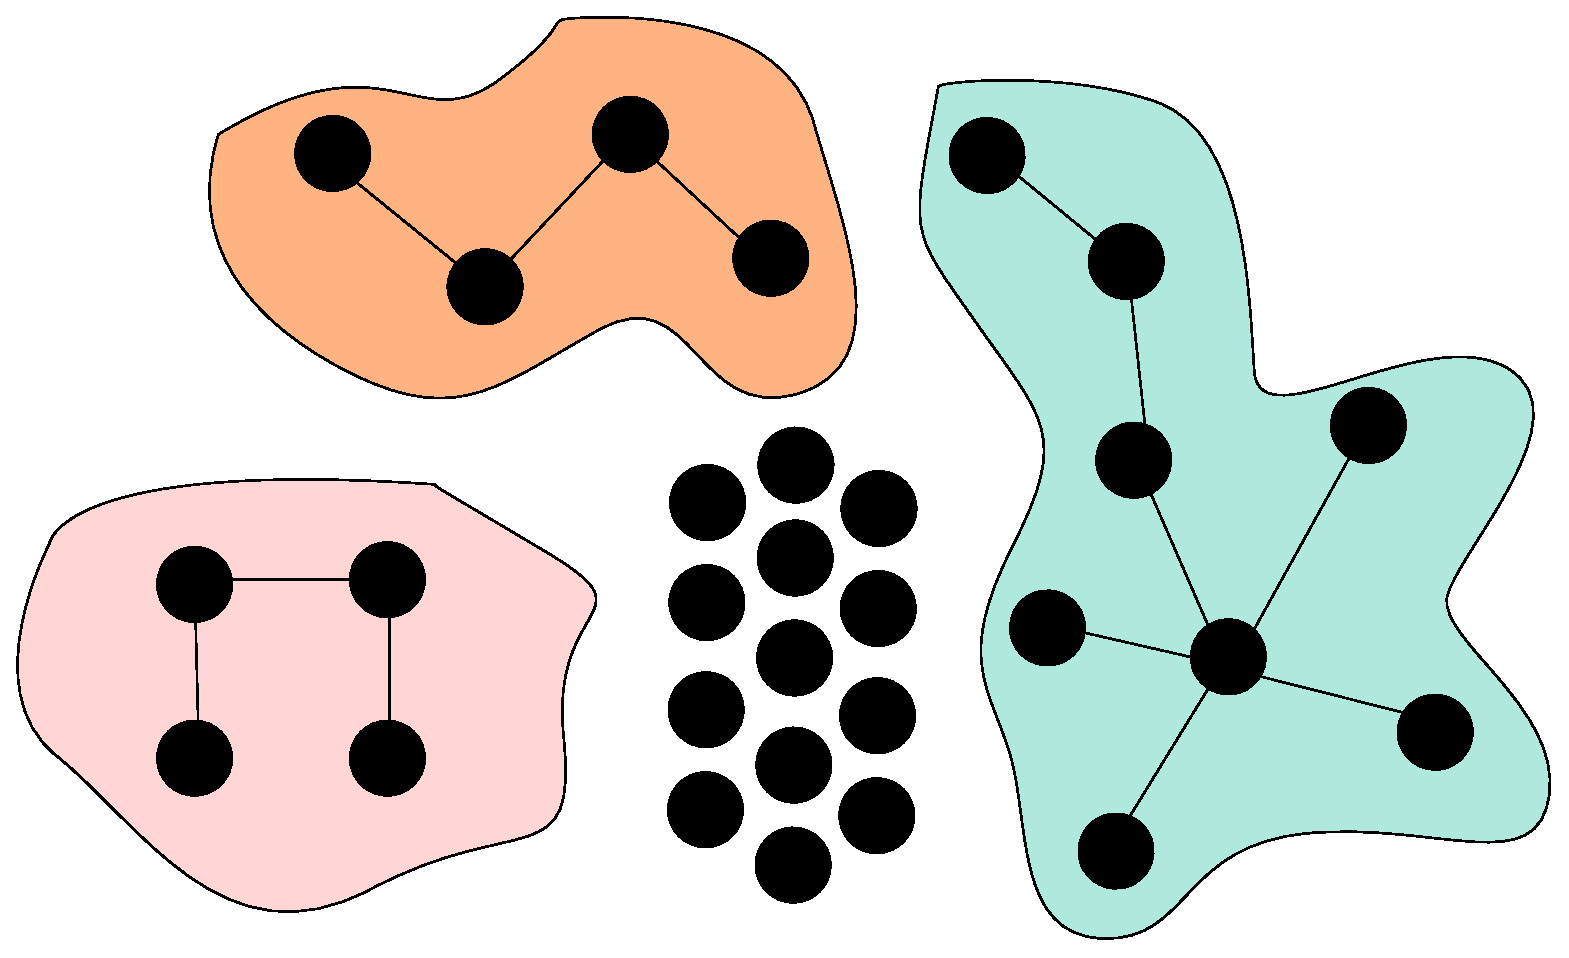
\includegraphics[width=\textwidth]{transitiveclosure}
% Clustering topics (black dots) by Transitive Closure based on similarity (arcs)
% \end{center}

%\igninetycap{transitiveclosure}{Clustering topics (black dots) by Transitive Closure based on similarity (arcs)}
\igonecap{transitiveclosure}{Clustering topics (black dots) by Transitive Closure based on similarity (arcs)}

\end{itemize}
\end{itemize}
\sslide{Case Study: Portability}
\begin{itemize}
\item MySQL 3.23 
	\begin{itemize}
	\item Discussions relating to portability
	\item Some topics smeared across multiple months


\newslide

%\begin{table*}
\begin{specquotef}
\centering
\begin{tabular}{|ccc|l|}

%\hline
%2000 &	Jul &	31 &		chmod \\
%2000 &	Sep &	29 &		fixes benchmark logging windows \\
%2000 &	Nov &	28 &		typo fix insert\_multi\_value \\
%2001 &	Jan &	27 &		fixes Innobase Cleanups auto-union \\
%2001 &	Mar &	28 &		2 topics bugfix, logging , TEMPORARY,	\\
\hline
2001 &	Jul &	26 &		update Allow TABLES LOCK [a] \\ 

2001 &	Aug &	25 &		tables row version [a] \\
\hline
%2001 &	Sep &	24 &		update checksum merge \\
%2001 &	Oct &	24 &		fixed fix \\
%2001 &	Dec &	23 &		HPUX SCO fix \\
\hline
2002 &	Feb &	21 &		net buffer length	max\_allowed\_packet [b] \\
2002 &	Mar &	23 &		small buf fix [b]	\\
%\hline
%2002 &	May &	22 &		[popular] fix SCO OSF1 table\_name \\
%2002 &	Nov &	18 &		HPUX11 compiler HP \\
\hline
\hline
2003 &	Feb &	16 &		Linux errno	[c] \\
2003 &	Mar &	18 &		alarm bookmark bug [c] \\
%\hline
%2003 &	Sep &	14 &		Auto logging merge windows distribution fix 64-bit 4.0 Cleanup \\
\hline
\end{tabular} \\
%\caption{Continuous blocks found while tracking topics associated with the word portability in MySQL 3.23}
{Continuous blocks found while tracking topics associated with the word portability in MySQL 3.23}
\label{tab:portability}
%\end{table*}
\end{specquotef}

\newslide

% \begin{figure}
%	 \centering
%	 \includegraphics[width=1.5\textwidth]{lda}
%	 \caption{Example of topics extracked from MySQL 3.23}
%	 \label{fig:mysql323}
% \end{figure}

%\igbigslidecap{lda}{Example of topics extracted from MySQL 3.23}
%\igonecap{lda}{Example of topics extracted from MySQL 3.23}
%\igbigcapb{lda}{Example of topics extracted from MySQL 3.23}
%\igbigthirtycapb{lda}{Example of topics extracted from MySQL 3.23}
\igbigthirtyfivecapb{lda}{Example of topics extracted from MySQL 3.23}

\end{itemize}
\end{itemize}
\sslide{Observations}
\begin{itemize}
\item Topics could be named
	\begin{itemize}
	\item Certain words indicate a focus on
		\begin{itemize}
		\item Maintenance
		\item Bug Fixing
		\item Portability
		\item Potential 'ilities

	\end{itemize}
\end{itemize}
\end{itemize}
\sslide{Observations}
\begin{itemize}
\item Powerlaw distribution of repeating topic counts
	\begin{itemize}
	\item Most occured once
	\item A few were repeated 
		\begin{itemize}
		\item less than 10\% of topics reoccur

	\end{itemize}
\end{itemize}
\end{itemize}
\sslide{Unfinished}
\begin{itemize}
\item Total Topics versus Monthly Topics

\end{itemize}
\sslide{Future work}
\begin{itemize}
\item Extension, associate Trends or Topics with purpoes by using wordnet and Taxonomies of software quality 

\end{itemize}
\end{slide}


\end{document}
